% Options for packages loaded elsewhere
\PassOptionsToPackage{unicode}{hyperref}
\PassOptionsToPackage{hyphens}{url}
%
\documentclass[
]{article}
\usepackage{lmodern}
\usepackage{amssymb,amsmath}
\usepackage{ifxetex,ifluatex}
\ifnum 0\ifxetex 1\fi\ifluatex 1\fi=0 % if pdftex
  \usepackage[T1]{fontenc}
  \usepackage[utf8]{inputenc}
  \usepackage{textcomp} % provide euro and other symbols
\else % if luatex or xetex
  \usepackage{unicode-math}
  \defaultfontfeatures{Scale=MatchLowercase}
  \defaultfontfeatures[\rmfamily]{Ligatures=TeX,Scale=1}
\fi
% Use upquote if available, for straight quotes in verbatim environments
\IfFileExists{upquote.sty}{\usepackage{upquote}}{}
\IfFileExists{microtype.sty}{% use microtype if available
  \usepackage[]{microtype}
  \UseMicrotypeSet[protrusion]{basicmath} % disable protrusion for tt fonts
}{}
\makeatletter
\@ifundefined{KOMAClassName}{% if non-KOMA class
  \IfFileExists{parskip.sty}{%
    \usepackage{parskip}
  }{% else
    \setlength{\parindent}{0pt}
    \setlength{\parskip}{6pt plus 2pt minus 1pt}}
}{% if KOMA class
  \KOMAoptions{parskip=half}}
\makeatother
\usepackage{xcolor}
\IfFileExists{xurl.sty}{\usepackage{xurl}}{} % add URL line breaks if available
\IfFileExists{bookmark.sty}{\usepackage{bookmark}}{\usepackage{hyperref}}
\hypersetup{
  pdftitle={Data Processes Project Report},
  pdfauthor={Carlos Sanchez; Alvaro Arranz; Angel González; Daniel Saiz},
  hidelinks,
  pdfcreator={LaTeX via pandoc}}
\urlstyle{same} % disable monospaced font for URLs
\usepackage[margin=1in]{geometry}
\usepackage{longtable,booktabs}
% Correct order of tables after \paragraph or \subparagraph
\usepackage{etoolbox}
\makeatletter
\patchcmd\longtable{\par}{\if@noskipsec\mbox{}\fi\par}{}{}
\makeatother
% Allow footnotes in longtable head/foot
\IfFileExists{footnotehyper.sty}{\usepackage{footnotehyper}}{\usepackage{footnote}}
\makesavenoteenv{longtable}
\usepackage{graphicx,grffile}
\makeatletter
\def\maxwidth{\ifdim\Gin@nat@width>\linewidth\linewidth\else\Gin@nat@width\fi}
\def\maxheight{\ifdim\Gin@nat@height>\textheight\textheight\else\Gin@nat@height\fi}
\makeatother
% Scale images if necessary, so that they will not overflow the page
% margins by default, and it is still possible to overwrite the defaults
% using explicit options in \includegraphics[width, height, ...]{}
\setkeys{Gin}{width=\maxwidth,height=\maxheight,keepaspectratio}
% Set default figure placement to htbp
\makeatletter
\def\fps@figure{htbp}
\makeatother
\setlength{\emergencystretch}{3em} % prevent overfull lines
\providecommand{\tightlist}{%
  \setlength{\itemsep}{0pt}\setlength{\parskip}{0pt}}
\setcounter{secnumdepth}{-\maxdimen} % remove section numbering

\title{Data Processes Project Report}
\author{Carlos Sanchez \and Alvaro Arranz \and Angel González \and Daniel Saiz}
\date{12/16/2019}

\begin{document}
\maketitle

\hypertarget{introduction-and-related-work}{%
\subsubsection{Introduction and Related
Work}\label{introduction-and-related-work}}

On the project proposal we formulated 3 different questions. We decide
to answer the second one about the gap between east and west
conferences.

One of our member followed for years the NBA and during that period of
time the Western conference teams ruled the league with Golden State
Warriors on the head. Only the Cleveland Cavaliers and Miami Heat,
thanks to LeBron James could fight against the best western team. During
the last 8 seasons, LeBron James won 4 rings (3 with Miami Heats and 1
with Cleveland Cavaliers) and played 7 finals.

LeBron James is one of the best players in the NBA history, and he is
able to lead a whole team to the victory almost by himself, but this is
not the case with any other player of the league at this moment. LeBron
moved to Los Angeles Lakers on the last season, and the project wasn't
complete, which is one of the reasons to select the season 2018/2019 to
avoid an outlier on the eastern team where LeBron is playing.

To check if we were sure about our assumptions, we loaded the Match
Statistics Dataset and performed several transformations to retrieve the
data we wanted.

\begin{longtable}[]{@{}lr@{}}
\toprule
Conference & Wins\tabularnewline
\midrule
\endhead
EAST & 198\tabularnewline
WEST & 252\tabularnewline
\bottomrule
\end{longtable}

It seems like the gap between the West and the East is still there, but
with this simple table we cannot be sure the data is not biased by low
performing teams. To check this we plotted the wins against teams of the
same conference and teams of the other, clustering the results by
conferences. The script which generates the following chart can be found
\href{https://github.com/AlmaProcesses/NBA_Project/blob/master/question_2.R}{here}

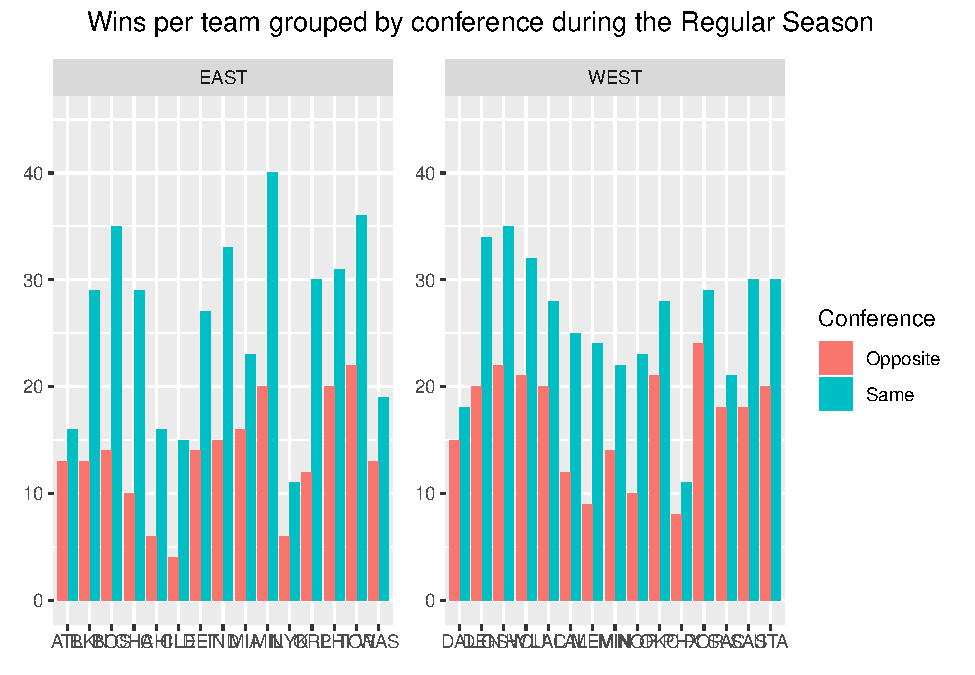
\includegraphics{index_files/figure-latex/patchwork-1.pdf}

We can see how West teams perform better than East ones on the cross
matches. The eastern team with the most victories during the regular
season was Toronto Raptors, which finally won the playoffs finals
against Golden State Warriors. With this visualization we can assure the
West conference was stronger than the East conference during the season
2018/2019.

Here you will find several relevant work about this question that we
want to answer:

\begin{itemize}
\tightlist
\item
  \href{https://thegruelingtruth.com/basketball/the-talent-difference-between-the-west-and-eastern-conferences/}{The
  Talent Difference Between the West and Eastern Conferences}
\item
  \href{http://pagines.uab.cat/appliedeconomics/sites/pagines.uab.cat.appliedeconomics/files/Brosed,\%20M._paper.pdf}{COMPETITIVE
  BALANCE IN THE NBA: Comparative analysis of Eastern and Western
  Conferences}
\item
  \href{https://www.sbnation.com/nba/2019/10/22/20899122/nba-predictions-2019-2020-season-mvp-championship-nba-finals-lakers-clippers}{NBA
  Predictions for the 2019-2020 Season}
\end{itemize}

\hypertarget{exploratory-data-analysis}{%
\subsubsection{Exploratory Data
Analysis}\label{exploratory-data-analysis}}

\hypertarget{datasets}{%
\paragraph{Datasets}\label{datasets}}

The dataset has been produced using the R package
\href{http://asbcllc.com/nbastatR/}{nbastatR}, which parses information
from the official \href{https://stats.nba.com/}{NBA API} and different
pages containing NBA historic data like
\href{https://hoopshype.com/}{Hoopshype.com}. There are two different
datasets:

\hypertarget{match-statistics-dataset}{%
\subparagraph{Match Statistics Dataset}\label{match-statistics-dataset}}

This dataset contains statistics about the NBA games during the 2018-19
season.

This dataset consists of one csv file. It's named
\href{https://github.com/AlmaProcesses/NBA_Project/blob/master/data/regularseason1819_games.csv}{regularseason1819\_games.csv}.
It has 2460 observations and 47 features.

\begin{longtable}[]{@{}lll@{}}
\toprule
Column & Type & Description\tabularnewline
\midrule
\endhead
\texttt{yearSeason} & num & The year when the statistics were
taken\tabularnewline
\texttt{slugSeason} & num & The season of the match\tabularnewline
\texttt{slugLeague} & chr & League name abbreviation\tabularnewline
\texttt{typeSeason} & chr & Type of season (always
\texttt{Regular\ Season})\tabularnewline
\texttt{dateGame} & date & Date the match was played\tabularnewline
\texttt{idGame} & num & Id of the match on the NBA API\tabularnewline
\texttt{numberGameTeamSeason} & num & Match order for the
team\tabularnewline
\texttt{nameTeam} & num & Name of the team\tabularnewline
\texttt{idTeam} & num & Id of the team on the NBA API\tabularnewline
\texttt{isB2B} & logi & The match was a back to back\tabularnewline
\texttt{isB2BFirst} & logi & The match was the first back to
back\tabularnewline
\texttt{isB2BSecond} & logi & The match was the second back to
back\tabularnewline
\texttt{locationGame} & chr & Location where the match was
played\tabularnewline
\texttt{slugMatchup} & chr & Abbreviation of the match\tabularnewline
\texttt{slugTeam} & chr & Abbreviation of the team\tabularnewline
\texttt{countDaysRestTeam} & num & Days the team had for resting before
the match\tabularnewline
\texttt{countDaysNextGameTeam} & num & Days before the next team's
match\tabularnewline
\texttt{slugOpponent} & chr & Abbreviation of the opponent
team\tabularnewline
\texttt{slugTeamWinner} & chr & Abbreviation of the winner
team\tabularnewline
\texttt{slugTeamLoser} & chr & Abbreviation of the defeated
team\tabularnewline
\texttt{outcomeGame} & chr & The abbreviation of the result
(\texttt{W\textbar{}L})\tabularnewline
\texttt{isWin} & logi & True if the team won the match\tabularnewline
\texttt{fgmTeam} & num & Field goals made by the team\tabularnewline
\texttt{fgaTeam} & num & Field goals attempted by the
team\tabularnewline
\texttt{pctFGTeam} & num & \% of field goals made vs
attempted\tabularnewline
\texttt{fg3mTeam} & num & 3-pts field goals made by the
team\tabularnewline
\texttt{fg3aTeam} & num & 3-pts field goals attempted by the
team\tabularnewline
\texttt{pctFG3Team} & num & \% of 3-pts field goals made vs
attempted\tabularnewline
\texttt{pctFTTeam} & num & \% of free throws scored\tabularnewline
\texttt{hasVideo} & logi &\tabularnewline
\texttt{fg2mTeam} & num & 2-pts field goals made by the
team\tabularnewline
\texttt{fg2aTeam} & num & 2-pts field goals attempted by the
team\tabularnewline
\texttt{pctFG2Team} & num & \% of 2-pts field goals attempted by the
team\tabularnewline
\texttt{minutesTeam} & num & Minutes played by the team\tabularnewline
\texttt{ftmTeam} & num & Free throws made by the team\tabularnewline
\texttt{ftaTeam} & num & Free throws attempted by the
team\tabularnewline
\texttt{orebTeam} & num & Offensive rebounds of the team\tabularnewline
\texttt{drebTeam} & num & Defensive rebounds of the team\tabularnewline
\texttt{trebTeam} & num & Total rebounds of the team\tabularnewline
\texttt{astTeam} & num & Number of assists of the team\tabularnewline
\texttt{stlTeam} & num & Number of steals of the team\tabularnewline
\texttt{blkTeam} & num & Number of blocks of the team\tabularnewline
\texttt{tovTeam} & num & Number of turnovers of the team\tabularnewline
\texttt{pfTeam} & num & Number of personal fouls of the
team\tabularnewline
\texttt{ptsTeam} & num & Points scored by the team\tabularnewline
\texttt{plusminusTeam} & num & Difference of points scored with the
other team\tabularnewline
\texttt{urlTeamSeasonLogo} & chr & Url with the logo of the
team\tabularnewline
\bottomrule
\end{longtable}

\hypertarget{teams-dataset}{%
\subparagraph{Teams Dataset}\label{teams-dataset}}

This dataset contains information about the Teams in the NBA.

This dataset consists of one csv file. The first one,
\href{https://github.com/AlmaProcesses/NBA_Project/blob/master/data/nba_teams.csv}{nba\_teams.csv},
is a list of the teams of the NBA and their information. It has 30
observations and 9 features.

\begin{longtable}[]{@{}lll@{}}
\toprule
Column & Type & Description\tabularnewline
\midrule
\endhead
\texttt{nameTeam} & chr & Name of the team\tabularnewline
\texttt{idTeam} & num & Id of the team\tabularnewline
\texttt{slugTeam} & chr & The acronym of the
\texttt{nameTeam}\tabularnewline
\texttt{teamName} & chr & The colloquial name of the
\texttt{nameTeam}\tabularnewline
\texttt{cityTeam} & chr & Name of the City where the team
belongs\tabularnewline
\texttt{teamNameFull} & chr & The abbreviation of the
\texttt{nameTeam}\tabularnewline
\texttt{idConference} & num & Id of the team conference\tabularnewline
\texttt{idDivision} & num & Id of the team division\tabularnewline
\texttt{urlThumbnailTeam} & chr & Url with the logo of the
team\tabularnewline
\bottomrule
\end{longtable}

\begin{itemize}
\tightlist
\item
  Creates 5 well designed and formatted graphics (\textbf{15 points}, 3
  each)

  \begin{itemize}
  \tightlist
  \item
    The visual uses the appropriate visual encodings based on the data
    type (\textbf{1 point})
  \item
    Written interpretation of graphic is provided (\textbf{1 point})
  \item
    Clear axis labels, titles, and legends are included, where
    appropriate (\textbf{1 point})
  \end{itemize}
\end{itemize}

\hypertarget{methods-30-points}{%
\subsubsection{\texorpdfstring{Methods (\textbf{30
points})}{Methods (30 points)}}\label{methods-30-points}}

The appropriate methods are employed to answer the question of interest,
including: - \textbf{Strength of relationships}: Uses the appropriate
technique to assess the strength of relationships amongst your variables
of interest. You should include: - A formula describing how you believe
your features (independent variables) are related to your outcome of
interest (dependent variable) (\textbf{5 points}) - A defense of the
variables included in your formula (\textbf{5 points}) - Creating the
appropriate model based on your dataset (\textbf{5 points})

\begin{itemize}
\tightlist
\item
  \textbf{Prediction}: You must also make predictions for your outcome
  of interest. In doing so, you must demonstrate a clear use of:

  \begin{itemize}
  \tightlist
  \item
    Splitting your data into testing/training data (\textbf{2 points})
  \item
    Applying cross validation to your model (\textbf{3 points})
  \item
    Appropriately handling any missing values (\textbf{2 points})
  \item
    Appropriately using categorical variables (\textbf{3 points})
  \item
    Using a grid search to find the best parameters for you model of
    interest (\textbf{2 points})
  \item
    Employing the algorithm of interest (\textbf{3 points})
  \end{itemize}
\end{itemize}

\hypertarget{results-20-points}{%
\subsubsection{\texorpdfstring{Results (\textbf{20
points})}{Results (20 points)}}\label{results-20-points}}

You must provide a clear interpretation of your statistical and machine
learning results, including at least \textbf{one visual or table} for
each. - \textbf{Strengths of relationships}: For the features you
included in your model, you must describe the strength (significance)
and magnitude of the relationships. This can be presented in a table or
chart, and pertinent observations should be described in the text.
(\textbf{10 points}) - \textbf{Predictions}: How well were you able to
predict values in the dataset? You should both report appropriate
metrics based on the type of outcome you're predicting (e.g., root mean
squared error v.s. accuracy), as well as a high quality visual showing
the strength of your model (\textbf{10 points})

\hypertarget{discussion-and-future-work-10-points}{%
\subsubsection{\texorpdfstring{Discussion and Future Work (\textbf{10
points})}{Discussion and Future Work (10 points)}}\label{discussion-and-future-work-10-points}}

Based on \emph{specific observations} from the results section, the
report clearly provides: - An analysis of the real world implications of
the results, at least one full paragraph (\textbf{5 points}) - Clear
suggestion for directions of future research, at least one full
paragraph (\textbf{5 points})

\end{document}
